\documentclass[aspectratio=169]{beamer}
\usepackage{tikz}
\usepackage{graphicx}
\usepackage{listings}
\usepackage{xcolor}
\usepackage{hyperref}
\usepackage[spanish,es-noquoting]{babel}

\lstset{
  basicstyle=\ttfamily\small,
  keywordstyle=\color{blue},
  stringstyle=\color{red},
  commentstyle=\color{gray},
  showstringspaces=false
}
% Minimal look
\usetheme{Warsaw}
%\setbeamertemplate{headline}
\setbeamertemplate{footline}{
  \leavevmode%
  \hbox{%
    % Left: Section name
    \begin{beamercolorbox}[wd=.33\paperwidth,ht=2.25ex,dp=1ex,left]{author in head/foot}%
      \hspace*{2ex}\insertsection
    \end{beamercolorbox}%
    % Center: Presentation title
    \begin{beamercolorbox}[wd=.34\paperwidth,ht=2.25ex,dp=1ex,center]{title in head/foot}%
      \insertshorttitle
    \end{beamercolorbox}%
    % Right: Slide numbers
    \begin{beamercolorbox}[wd=.33\paperwidth,ht=2.25ex,dp=1ex,right]{date in head/foot}%
      \insertframenumber{} / \inserttotalframenumber\hspace*{2ex}
    \end{beamercolorbox}%
  }%
  \vskip0pt%
}

\usecolortheme{default}
\usefonttheme{serif}
\graphicspath{{../}{./}}
\setbeamertemplate{caption}[numbered]

% Title info
\title[LegalAI Presentation]{LegalAI Presentation}
\subtitle{}
\author{Ricardo Reyes-Jimenez}
\institute{Universidad de La Sabana}
\date{\today}

% Background image for title slide
\usebackgroundtemplate{
  \tikz\node[opacity=0.3]{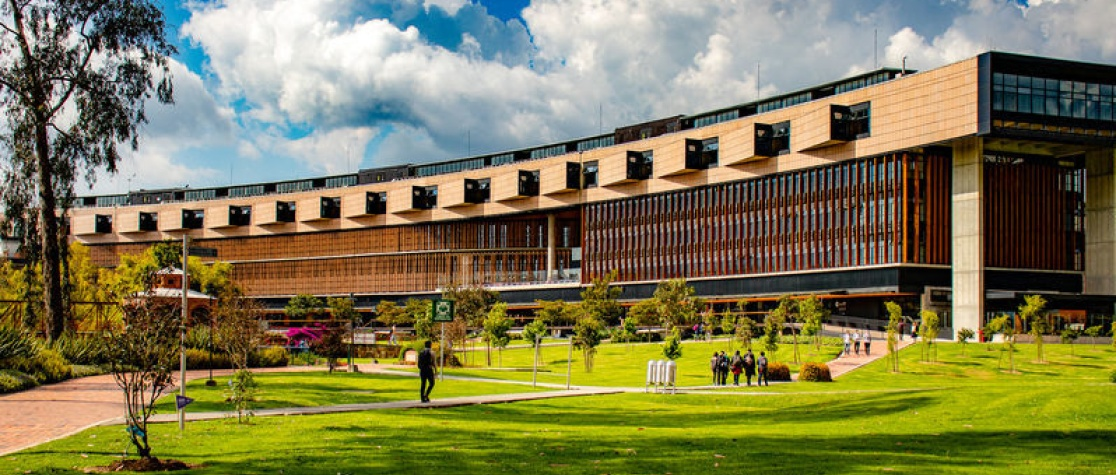
\includegraphics[width=\paperwidth,height=\paperheight]{Images/UniSabana.jpg}};
}

\begin{document}

% Title slide
\begin{frame}
  \titlepage
\end{frame}

% Reset background for normal slides
\usebackgroundtemplate{}


\begin{frame}{El Futuro en el Presente: IA y Derecho Laboral en Colombia}
## Una aventura legal y tecnológica para mentes curiosas
### Profesor Ricardo Reyes-Jiménez
#### \textit{Facultad de Estudios Jurídicos, Políticos e Internacionales - Universidad de la Sabana}
##### Hoy, en la Era de la Inteligencia Artificial
\end{frame}


\begin{frame}{¡Atención, futuros guardianes de la justicia!}
Imagina por un segundo... Estás trabajando, tranquilamente, cuando de repente, \textbf{¡BUM!} Un algoritmo decide tu horario, evalúa tu desempeño o, peor aún, te despide. ¿Ciencia ficción? ¡Para nada! Esto es la realidad que la Inteligencia Artificial nos está lanzando a la cara, especialmente en el vibrante mundo del Derecho Laboral colombiano.
Hoy, no solo vamos a hablar de leyes. ¡Vamos a explorar un campo de batalla legal donde los códigos se encuentran con los algoritmos!
\textbf{¿Listos para desentrañar este misterio digital?}
\end{frame}


\begin{frame}{La ola de la IA: ¿Amiga o enemiga?}
La Inteligencia Artificial ya no es solo para las películas. Está en nuestros celulares, en nuestras compras, ¡y sí, en nuestros trabajos! Pero, ¿qué significa realmente para el día a día de un trabajador o para las responsabilidades de un empleador en Colombia?
\textbf{Pregunta interactiva para la audiencia:}
\begin{itemize}
  \item \textbf{``Levanten la mano, ¿quién de ustedes ha interactuado con una IA hoy? ¿Siri? ¿ChatGPT? ¿Un filtro de Instagram? ¡Confiesen!''}
  \item (Esperar respuestas y comentarios)
\end{itemize}
La IA promete eficiencia, productividad... ¡pero también susurros de desempleo masivo y preguntas inquietantes sobre quién manda al final del día. `\cite{Gauthier, G. (2024)}`
\end{frame}


\begin{frame}{Colombia: En la primera línea digital}
Nuestro país, con su espíritu emprendedor y su gente trabajadora, no es ajeno a esta revolución. La IA ya está transformando sectores desde la manufactura hasta el servicio al cliente, y con ella, llegan desafíos legales \textbf{¡frescos y urgentes!}
La integración de la IA en el mercado laboral colombiano no solo está cambiando cómo trabajamos, sino que está creando ¡un nuevo campo de juego legal y ético! `\cite{Eljach Mendoza, C. (2024)}`
\textbf{Imagina esta historia:}
María trabaja en una fábrica de textiles en Medellín. Antes, su jefe le asignaba las tareas. Ahora, un sofisticado sistema de IA optimiza la producción, decide cuándo debe tomar un descanso e incluso evalúa su eficiencia en tiempo real. ¿Quién es el jefe de María? ¿El gerente humano o el algoritmo? ¿Y si el algoritmo está sesgado?
\end{frame}


\begin{frame}{Redefiniendo ``Trabajo'' y ``Trabajador'': ¡Un terremoto conceptual!}
El Derecho Laboral clásico se construyó sobre pilares como la \textbf{subordinación}, la \textbf{ajenidad} y la \textbf{prestación personal del servicio}. Pero, ¿qué pasa cuando una IA es la que da las órdenes? ¿O cuando un ``trabajador'' es en realidad un algoritmo que ejecuta tareas? `\cite{Otero, L. (2023)}`
\textbf{¡Sabías que...}
La IA no solo promete eficiencia, sino que nos obliga a redefinir qué es ``trabajo'' y quién es un ``empleado''. Las viejas definiciones que sustentan nuestro Derecho Laboral están siendo puestas a prueba por un mundo cada vez más automatizado.
\textbf{Pregunta interactiva para la audiencia:}
\begin{itemize}
  \item \textbf{``Si un algoritmo de IA gestiona tu horario, aprueba tus vacaciones y te da feedback sobre tu desempeño, ¿ese algoritmo es tu jefe? ¿Podríamos demandar a un algoritmo?''}
  \item (Pausa para reacciones y debate)
\end{itemize}
\end{frame}


\begin{frame}{Los Gigantes del Desafío: Implicaciones Legales}
La IA nos trae un festín de preguntas para los juristas:
### 1. Gestión Algorítmica: ¿El jefe sin corazón?
\begin{itemize}
  \item \textbf{Sesgos:} Si los datos de entrenamiento de la IA tienen prejuicios, ¿la IA discriminará en contratación o evaluación?
  \item \textbf{Transparencia:} ¿Cómo saber por qué una IA tomó una decisión sobre un trabajador? ¡El famoso ``derecho a la explicación''!
\end{itemize}
### 2. Privacidad de Datos en el Trabajo: ¿Ojo que todo lo ve?
\begin{itemize}
  \item La IA necesita datos. ¿Qué datos de los trabajadores son lícitos recolectar? ¿Monitoreo constante?
  \item ¿Cómo protegemos la información sensible de nuestros colaboradores?
\end{itemize}
\end{frame}


\begin{frame}{Los Gigantes del Desafío: Más allá de la Gestión}
### 3. Desplazamiento Laboral y Re-capacitación: ¿Sin trabajo o con nuevo trabajo?
\begin{itemize}
  \item La IA puede automatizar tareas repetitivas, pero también crea nuevas. ¿Estamos preparando a la fuerza laboral colombiana para estos nuevos roles?
  \item ¡Es crucial el reentrenamiento! No es el fin del trabajo, es el fin \textit{de cierto tipo} de trabajo. `\cite{Gauthier, G. (2024)}`
\end{itemize}
### 4. Responsabilidad: ¿Quién paga los platos rotos?
\begin{itemize}
  \item Si una IA causa un daño (por ejemplo, al tomar una decisión que viola un derecho laboral), ¿quién es el responsable? ¿El desarrollador? ¿El empleador que la implementó? ¿La IA misma (personalidad jurídica para IA)? ¡Un laberinto legal!
\end{itemize}
\end{frame}


\begin{frame}{¡Sabías que...!  (Nuestra sección de datos curiosos)}
Aquí les traigo un par de pepitas de oro de la investigación que hemos realizado:
\begin{itemize}
  \item \textbf{La Nueva Frontera Legal:} La vertiginosa integración de la IA en el mercado laboral colombiano no solo está desarmando las estructuras de empleo tradicionales, sino que nos está lanzando ¡desafíos legales y éticos totalmente nuevos! Esto nos obliga a una reevaluación \textbf{urgente} de nuestras leyes para abordar temas como la gestión algorítmica, la privacidad de datos y la equidad en la contratación. ¡Estamos en una verdadera carrera contra el tiempo! `\cite{Eljach Mendoza, C. (2024)}`
  \item \textbf{¿Qué es un ``Trabajador'' en la Era IA?} Mientras la IA nos promete cielos de eficiencia, también nos bombardea con preguntas existenciales sobre la pérdida de empleos y la necesidad imperante de que los trabajadores se re-capaciten. Pero aún más fundamental, ¡está desafiando las mismísimas definiciones de ``trabajo'' y ``empleado'' que han sido el corazón del Derecho Laboral colombiano! Es hora de nuevas interpretaciones y protecciones en este mundo cada vez más automatizado. `\cite{Otero, L. (2023)}`
\end{itemize}
\end{frame}


\begin{frame}{El Futuro es Ahora: Adaptación e Innovación}
Entonces, ¿qué hacemos? ¿Nos escondemos bajo una piedra? ¡Claro que no! Como juristas y futuros líderes, tenemos una misión:
\begin{itemize}
  \item \textbf{Actualizar Marcos Regulatorios:} Necesitamos leyes ágiles que protejan a los trabajadores sin ahogar la innovación. ¡Un equilibrio delicado!
  \item \textbf{Formación y Re-capacitación:} Invertir en el capital humano para que la IA sea una herramienta, no un reemplazo total.
  \item \textbf{Diálogo Multisectorial:} Abogados, tecnólogos, empresarios, trabajadores, ¡todos a la mesa para construir el futuro juntos!
\end{itemize}
\textbf{La Inteligencia Artificial no es una moda pasajera; es una fuerza transformadora.} Nuestro desafío no es luchar contra ella, sino integrarla con sabiduría, ética y, sobre todo, justicia.
\end{frame}


\begin{frame}{Conclusión: ¡El Código y el Algoritmo!}
Hemos navegado por el apasionante, y a veces intimidante, mundo del impacto de la IA en el Derecho Laboral colombiano.
\begin{itemize}
  \item Hemos visto cómo redefine conceptos clásicos.
  \item Hemos explorado los desafíos de la gestión algorítmica, la privacidad y la responsabilidad.
  \item Y hemos recordado que, como sociedad, tenemos el poder de moldear este futuro.
\end{itemize}
El Derecho Laboral no está muriendo; ¡está evolucionando! Y necesitamos mentes brillantes como las suyas para guiar esa evolución con visión, empatía y conocimiento.
\textbf{¡Gracias por ser parte de esta conversación crucial!}
\end{frame}


\begin{frame}{¿Preguntas para el Profesor?}
¡Estoy listo para el debate, las dudas y las ideas brillantes que seguro tienen!
\end{frame}


\begin{frame}{Referencias}
\begin{itemize}
  \item \textbf{Eljach Mendoza, C.} (2024). ``Impacto social y jurídico de la inteligencia artificial en el mercado laboral colombiano''. \textit{Saber, Ciencia y Libertad en Germinación}, \textit{17}. DOI: 10.18041/2382-3755/germinacion.2024v17.12207
  \item \textbf{Gauthier, G.} (2024). ``El impacto de la inteligencia artificial en el trabajo''. \textit{Derecho Laboral. Revista de doctrina, jurisprudencia e informaciones sociales}. DOI: 10.59709/der.lab.2024.294-295.3
  \item \textbf{Otero, L.} (2023). ``EL IMPACTO DE LA INTELIGENCIA ARTIFICIAL EN LAS CATEGORÍAS CLÁSICAS DEL DERECHO DEL TRABAJO''. \textit{Derecho, nuevas tecnologías e Inteligencia Artificial}. DOI: 10.2307/jj.13286115.20
\end{itemize}
\end{frame}



\begin{frame}[allowframebreaks]{Referencias}
  \bibliographystyle{apalike}
  \bibliography{references}
\end{frame}

\end{document}